\documentclass[12pt,a4paper]{article}
\usepackage[utf8]{inputenc}
\usepackage[russian]{babel}
\usepackage[OT1]{fontenc}
\usepackage{amsmath}
\usepackage{amsfonts}
\usepackage{amssymb}
\usepackage{graphicx}
\graphicspath{{Images/}}
\usepackage[left=2cm,right=2cm,top=2cm,bottom=2cm]{geometry}
\usepackage{calc}
\usepackage{wrapfig}
\usepackage{setspace}
\usepackage{indentfirst}
\usepackage{subfigure}
\usepackage{multirow}


\title{
1.3.3.

Измерение вязкости воздуха по течению
в тонких трубках
}

\author{Семёнов Андрей Б02-016}

\begin{document}

\date{25 марта 2021г.}
\maketitle
\newpage

\textbf{Цель работы:} экспериментально исследовать свойства течения газов по тонким трубкам при различных числах Рейнольдса; выявить область применимости закона Пуазейля и с его помощью определить коэффициент вязкости воздуха.

\textbf{В работе используются:} система подачи воздуха (компрессор, поводящие трубки); газовый счетчик барабанного типа; спиртовой микроманометр с регулируемым наклоном; набор трубок различного диаметра с выходами для подсоединения микроманометра; секундомер

\section{Теоретический материал}

Работа посвящена изучению течения воздуха по прямой трубе круглого сечения. Движение жидкости или газа вызывается перепадом внешнего давления на концах $\Delta P$ трубы, чему в свою очередь препятствуют силы вязкого (внутреннего) трения, действующие между соседними слоями жидкости, а также со стороны стенок трубы.

Сила вязкого трения как в жидкостях, так и в газах описывается законом
Ньютона: касательное напряжение между слоями пропорционально перепаду
скорости течения в направлении, поперечном к потоку. В частности, если жидкость течёт вдоль оси x,  а скорость течения $v_{x}(y)$ зависит от координаты $y$  в каждом слое возникает направленное по $x$ касательное напряжение.

Величину $\eta$ называют коэффициентом динамической вязкости (или просто вязкостью) среды.

Объёмным расходом (или просто расходом) $Q$ называют объём жидкости,
протекающий через сечение трубы в единицу времени. Величина $Q$ зависит от
перепада давления $\Delta P$, а также от свойств газа (плотности $\rho$ и вязкости $\eta$) и от
геометрических размеров (радиуса трубы $R$ и её длины $L$). Основная задача
данной работы — исследовать эту зависимость экспериментально.

Характер течения в трубе может быть ламинарным либо турбулентным. 

Характер течения определяется безразмерным параметром задачи — числом Рейнольдса

$$ Re = \frac{\rho u a}{\eta}$$, где

$\rho$ - плотность жидкости, $u$ - скорость движения потока, $a$ - характерный размер потока.

Выпишем некоторые теоретические зависимости:

$$P(x) = P_{0} - \frac{\Delta P}{l}x$$

$$u = \frac{Q}{\pi R^{2}} = \frac{U_{max}}{2}$$

$$Q = \frac{\pi R^{4} \Delta P}{8\eta l}$$

$$l_{\text{уст}} \approx 0,2R\cdot Re$$
\newpage

\section{Экспериментальная установка}

\begin{figure}[h!]
	\begin{center}
		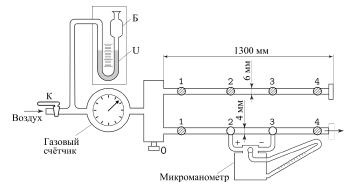
\includegraphics[width = 0.85\textwidth]{Scem_of_facility}
		\caption{Схема экспериментальной установки}
		\label{fig:facility}
	\end{center}
\end{figure}

\section{Выполнение работы}


\end{document}